% Abstract for the SEG 2012 Meeting
% Authors: Leonardo Uieda and Valeria C. F. Barbosa

\documentclass{segabs}
\usepackage{bibentry}
\usepackage{amsmath}

% Math commands
\newcommand{\vect}[1]{\mathbf{#1}}
\newcommand{\mat}[1]{\mathbf{#1}}

% Use \begin{sloppypar} so that some words like numbers and dates don't stick
% out of the text

\title{Use of the ``shape-of-anomaly'' data misfit in 3D 
inversion by planting anomalous densities}

\renewcommand{\thefootnote}{\fnsymbol{footnote}} 

\author{Leonardo Uieda\footnotemark[1] and Val\'eria C. F. Barbosa,
Observat\'orio Nacional}

\footer{}
\lefthead{Uieda \& Barbosa}
\righthead{``Shape-of-anomaly'' 3D inversion}


\begin{document}

\maketitle

\begin{abstract}
We present an improvement to the method of 3D gravity gradient inversion by
planting anomalous densities.
This method estimates a density-contrast distribution defined on a grid of
right-rectangular prisms.
Instead of solving large equation systems, the method uses a systematic search
algorithm to grow the solution, one prism at a time, around user-specified
prisms called ``seeds''.
These seeds have known density contrasts and the solution is constrained to be
concentrated around the seeds as well as have their density contrasts.
Thus, prior geologic and geophysical information are incorporated into the
inverse problem through the seeds.
However, this leads to a strong dependence of the solution on the correct
location, density contrast, and number of seeds used.
Our improvement to this method consists of using the ``shape-of-anomaly''
data-misfit function in conjunction with the $\ell_{2}$-norm data-misfit
function.
The shape-of-anomaly function measures the different in shape between the
observed and predicted data and is insensitive to differences in amplitude.
Tests on synthetic and real data show that the improved method not only has an
increased robustness with respect to the number of seeds and their locations,
but also provides a better fit of the observed data.
\end{abstract}

\section{Introduction}

\begin{sloppypar}
Methods for the 3D inversion of potential field data can be divided into two
main categories: those that estimate the values of physical properties and those
that estimate the form of the sources, given their physical property values.
Examples from the category that estimates physical property values
include \citet{Bear1995}, \citet{Li1998a}, and \citet{Portniaguine1999}.
The category that estimates the form of the sources can be subdivided into
non-linear and linear methods.
Non-linear methods generally parametrize the form of the sources using prisms
with polygonal cross-section \citep[e.g.,][]{Radhakrishna1996, OliveiraJr2011}
or polyhedra \citep[e.g.,][]{Wildman2009}.
On the other hand, linear methods parametrize the subsurface using right
rectangular prisms \citep[e.g.,][]{Camacho2000, Krahenbuhl2006, SilvaDias2009,
SilvaDias2011, Uieda2011}.
The method of \citet{Uieda2011} implements a systematic search algorithm to
iteratively ``grow'' the solution around use-specified prisms called ``seeds''.
This method is based on the 2D approach of \citet{Rene1986} and uses the
regularizing function of \citet{SilvaDias2009} to impose compactness on the
solution.
The method is computationally efficient due to the implementation of a ``lazy
evaluation'' of the sensitivity matrix.
However, it is highly dependent on the number of seeds and the correct choice
of their locations and density contrasts.
We present an improvement to the method of \citet{Uieda2011} which uses the
``shape-of-anomaly'' data-misfit function of \citet{Rene1986} together with the
traditional $\ell_{2}$-norm data-misfit function.
Tests on synthetic and real data show the improved robustness of our method with
respect to the location and number of seeds.
\end{sloppypar}

\section{Methodology}

\begin{sloppypar}
Let us assume that there are $N_{c}$ types of observations available (e.g.,
the gravitational attraction and/or some combination of the components of the
gravity gradient tensor).
Now, let $\vect{g}^{\thinspace k}$, $k=1,\ldots,N_{c}$, be a vector with
$L$ observations of one of these types of data.
We assume that $\vect{g}^{\thinspace k}$ is caused by an anomalous density
distribution in the subsurface.
We discretize the subsurface into an interpretative model consisting of $M$
juxtaposed right rectangular prisms with homogeneous densities.
It follows that $\vect{g}^{\thinspace k}$ can be approximated by the sum of the
contribution of each prism.
In matrix notation, this relation is given by

\begin{equation}
    \vect{d}^{\thinspace k} = \mat{A}^{k}~\vect{p},
    \label{eq:forward}
\end{equation}

where $\vect{d}^{\thinspace k}$, $k=1,\ldots,N_{c}$, is the $L$-dimensional
predicted data vector,
$\vect{p}$ is the $M$-dimensional parameter vector whose $j$th element is the
density of the $j$th prism, and $\mat{A}^{k}$, $k=1,\ldots,N_{c}$, is the
$L \times M$ sensitivity matrix.
The elements of the sensitivity matrix can be calculated using the formula of
\citet{Nagy2000}.
\\[0.2cm]
The misfit between $\vect{g}^{\thinspace k}$ and $\vect{d}^{\thinspace k}$ can
be expressed through the normalized $\ell_{2}$-norm data-misfit function

\begin{equation}
    \phi^{k}(\vect{p}) = \sqrt{
    \dfrac{
        \sum\limits_{i=1}^{L}
        \left( g_{i}^{\thinspace k} - d_{i}^{\thinspace k} \right)^{2}
    }{
        \sum\limits_{i=1}^{L}\left(g_{i}^{\thinspace k}\right)^{2}}}.
    \label{eq:phik}
\end{equation}

Another measure of this misfit is the ``shape-of-anomaly'' function of
\citet{Rene1986}

\begin{equation}
    \psi^{\thinspace k}(\vect{p}) = \sqrt{
        \sum\limits_{i=1}^{L}
        \left(\alpha^{\thinspace k} g_{i}^{\thinspace k} - d_{i}^{\thinspace k}
        \right)^{2}
    }, 
    \label{eq:shapek}
\end{equation}

where $\alpha^{\thinspace k}$, $k=1,\ldots,N_{c}$, is a scale factor.
The shape-of-anomaly function, as its name suggests, measures only the
difference in shape between the observed and predicted data.
If the two data have the same shape, they will differ only by a factor of
$\alpha^{\thinspace k}$.
Thus, the optimum value for $\alpha^{\thinspace k}$ is the one that minimizes
$\psi^{\thinspace k}$ (equation \ref{eq:shapek}) \citep{Rene1986}.
For a given predicted data vector $\vect{d}^{\thinspace k}$
(equation \ref{eq:forward}), the value of
$\alpha^{\thinspace k}$ is calculated by differentiating $\psi^{\thinspace k}$
with respect to $\alpha^{\thinspace k}$ and equating the result to zero,
i.e.,

\begin{equation}
    \dfrac{\partial \psi^{\thinspace k}}{\partial \alpha^{\thinspace k}} =
    \dfrac{\alpha^{\thinspace k}
        \sum\limits_{i=1}^{L}\left(g_{i}^{\thinspace k}\right)^{2} +
        \sum\limits_{i=1}^{L} g_{i}^{\thinspace k}d_{i}^{\thinspace k}}
        {\sqrt{\sum\limits_{i=1}^{L}
        \left(\alpha^{\thinspace k} g_{i}^{\thinspace k} - d_{i}^{\thinspace k}
        \right)^{2}}} = 0~.
\end{equation}

Hence, before evaluating function $\psi^{\thinspace k}$ (equation
\ref{eq:shapek}), $\alpha^{\thinspace k}$ can be calculated by \citep{Rene1986}

\begin{equation}
    \alpha^{\thinspace k} = \dfrac{
        \sum\limits_{i=1}^{L} g_{i}^{\thinspace k} d_{i}^{\thinspace k}
    }{
        \sum\limits_{i=1}^{L}\left( g_{i}^{\thinspace k}\right)^{2}
    }.
    \label{eq:alpha}
\end{equation}

We can then define the total data-misfit function as the sum of the individual
data-misfit functions (equation \ref{eq:phik}) of each type of data available,
i.e.,

\begin{equation}
    \Phi(\vect{p}) = \sum\limits_{k=1}^{N_{c}} \phi^{k}(\vect{p}),
    \label{eq:phi}
\end{equation}

and, likewise, total shape-of-anomaly function as

\begin{equation}
    \Psi(\vect{p}) = \sum\limits_{k=1}^{N_{c}} \psi^{\thinspace k}(\vect{p}).
    \label{eq:shape}
\end{equation}

From now on, we follow the methodology of \citet{Uieda2011}, in which the
solution is iteratively built by the accretion of prisms to user-specified
``seeds''.
These seeds are prisms of the interpretative model with given density contrasts.
Before the iterative growth process starts, all elements of the parameter vector
$\vect{p}$ are set to zero.
Next, the elements of $\vect{p}$ corresponding to the seeds are assigned the
density contrasts of the respective seeds (Figure~\ref{fig:sketch}a).
The growth process is then started.
An iteration of the growth process consists of attempting to grow, one at a
time, each of the $N_{s}$ seeds (Figure~\ref{fig:sketch}b).
A seed grows by attempting to perform the accretion of one of its neighboring
prisms (i.e., prisms that share a face).
We define the accretion of a prism as changing its density contrast from zero to
the density contrast of the respective seed undergoing the accretion.
In order to be chosen for accretion, a neighboring prism must satisfy two
criteria:

\begin{enumerate}
    \item The accretion of a prism must decrease the total data-misfit
    function $\Phi(\vect{p})$ (equation \ref{eq:phi}) and satisfy the condition
    \begin{equation}
        \dfrac{|\Phi_{(new)} - \Phi_{(old)}|}{\Phi_{(old)}} \ge \delta ,
        \label{eq:delta}
    \end{equation}
    where $\Phi_{(new)}$ is the value of $\Phi(\vect{p})$ evaluated with the
    prism included in the estimate, $\Phi_{(old)}$ is the previous value of 
    $\Phi(\vect{p})$, and $\delta$ is a small positive constant that controls
    how much the solution is allowed to grow.
    
    \item The accretion of a prism must produce the smallest value of the goal
    function $\Gamma(\vect{p})$ out of all other prisms that satisfy the first
    criterion. Unlike \citet{Uieda2011}, we define the goal function as    
    \begin{equation}
        \Gamma(\vect{p}) = \Psi(\vect{p}) + \mu\theta(\vect{p}),
        \label{eq:goal}
    \end{equation}
    where $\Psi(\vect{p})$ is the total shape-of-anomaly function (equation
    \ref{eq:shape}), $\mu$ is a regularizing parameter, and $\theta(\vect{p})$
    is a modified version of the regularizing function of \citet{Uieda2011}
    \begin{equation}
        \theta(\vect{p}) = \frac{1}{f} \sum\limits_{j=1}^{M}
        \dfrac{p_j}{p_j + \epsilon} l_{j},
        \label{eq:regul}
    \end{equation}
    where $p_{j}$, $j=1,\ldots,M$, is the $j$th element of parameter vector
    $\vect{p}$,
    $\epsilon$ is a small positive constant, $l_{j}$ is the distance between the
    $j$th prism and the seed which performed its accretion, and $f$ is a scaling
    factor equal to the mean extent of the interpretative model
    (the region in the subsurface to be interpreted).
    In practice, $\epsilon$ is not needed because one could simply sum $l_{j}$
    or zero when evaluating the regularizing function.
\end{enumerate}

If none of the neighboring prisms of a seed satisfy these criteria, the
seed does not grow during this iteration.
The growth process continues while at least one seed is able to grow
(Figure~\ref{fig:sketch}c).
\citet{Uieda2012} provide an animation of a growth process performed on
synthetic data using the method of \citet{Uieda2011}.
\\[0.2cm]
We emphasize that the full sensitivity matrices $\mat{A}^{k}$ are not needed
at any single time during the inversion process.
Therefore, the ``lazy evaluation'' of the sensitivity matrices
proposed in \citet{Uieda2011} is still possible
in our modified algorithm, making the inversion fast and memory efficient.
\\[0.2cm]
For clarity, the modified planting algorithm proposed here will be henceforth
referred to as the shape-of-anomaly planting algorithm.
\end{sloppypar}

\begin{figure}[htb]
    %\vspace{0.7cm}
    \includegraphics[width=\columnwidth]{sketch/algorithm}
     %\vspace{-0.6cm}
    \caption{
        2D sketch of three stages of the planting algorithm.
        In the upper panels, the black dots represent the observed data and
        the red line represents the predicted data produced by the current
        estimate.
        In the lower panels, the light gray grid of prisms represents the
        interpretative model, the color-filed prisms represent the current
        estimate, and the colored outlines represent the neighboring prisms of
        the current estimate.
        (a) Initial state with the user-specified seeds included in the estimate
        with their corresponding density contrasts and all other parameters set
        to zero.
        (b) End of the first growth iteration where two accretions took place,
        one for each seed.
        The neighboring prisms of each seed and the predicted data are updated.
        (c) Final estimate at the end of the algorithm.
        Modified from \citet{Uieda2011}.
    \label{fig:sketch}}
    %\vspace{-0.5cm}
\end{figure}

\section{Application to synthetic data}

\begin{sloppypar}
We tested the advantages of the shape-of-anomaly planting algorithm over the
method of \citet{Uieda2011} on synthetic noise-corrupted data of the $g_{zz}$
component of the gravity gradient tensor (Figure~\ref{fig:synthetic}a-b).
The synthetic data are produced by an elongated prismatic body with
density contrast of $1.0\ \mathrm{g/cm}^3$ (black frame in
Figure~\ref{fig:synthetic}c-d).
The data set contains 400 observations on a regular grid at 150 meter height and
were contaminated with pseudorandom Gaussian noise with zero mean and
2 E\"otv\"os standard deviation.
We applied both methods on this data set using an interpretative model
consisting of 50,000 prisms.
To yield adequate results, the method of \citet{Uieda2011} would need
several seeds correctly located along the strike of the source.
However, here we used only one seed (white dot in Figure~\ref{fig:synthetic}a-b)
in both inversions.
The depth of seed was 700 meters (center of the simulated body) for the method
of \citet{Uieda2011} and 300 meters (top of the simulated body) for the
shape-of-anomaly planting algorithm.
These values were the ones that yielded the best results for both methods.
We used inversion control variables $\mu = 10^{5}$ for \citet{Uieda2011},
$\mu = 0.2$ for shape-of-anomaly, and $\delta = 0.0005$ for both methods.
\\[0.2cm]
Figure~\ref{fig:synthetic}c-d shows the estimated density-contrast distributions
obtained using each method.
As expected, the method of \citet{Uieda2011} is not able to recover the correct
geometry of the true source given only one seed.
Moreover, the estimated density-contrast distribution
(Figure~\ref{fig:synthetic}c) is not entirely compact and the predicted data
presents a reasonable fit to the synthetic data (Figure~\ref{fig:synthetic}a).
Conversely, the shape-of-anomaly planting algorithm estimates a density-contrast
distribution (Figure~\ref{fig:synthetic}d) that not only approximately recovers
the geometry of the true source, but is fully compact and produces a better fit
of the data.
\end{sloppypar}

\begin{figure}[htb]
    %\vspace{-0.3cm}
    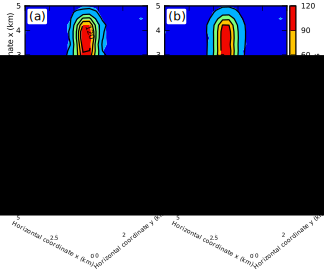
\includegraphics[width=\columnwidth]{synthetic/fig/synthetic}
     %\vspace{-0.6cm}
    \caption{Application to synthetic data. (a-b) Synthetic noise-corrupted
        (colored contours) and predicted (black contour lines)
        $g_{zz}$ components. White dots show the horizontal location
        of the seeds.
        (c-d) Perspective views of the estimated density-contrast distributions.
        a and c were produced by the method of \citet{Uieda2011} and
        b and d by the shape-of-anomaly planting algorithm.
        Red prisms have density contrast of $1.0\ \mathrm{g/cm}^3$.
        Prisms with density contrast of $0\ \mathrm{g/cm}^3$ are not shown.
        The black prismatic frame in c and d is the outline of the true source. 
    \label{fig:synthetic}}
    %\vspace{-0.5cm}
\end{figure}

\section{Application to real data}

\subsection{Quadril\'atero Ferr\'ifero}

\begin{sloppypar}
We applied the shape-of-anomaly planting algorithm to the gravity gradient
data from the Quadril\'atero Ferr\'ifero, Brazil.
We used the data of the $g_{yz}$ and $g_{zz}$ components in the inversion
(Figure~\ref{fig:qf}a) and assumed a density contrast of $1.0\ \mathrm{g/cm}^3$
between the iron ore and the host rocks \citep{Carlos2011, Uieda2011}.
The data set contains a total of 9164 measurements.
The interpretative model consists of 310,500 prisms which follow the topography
of the area.
We used five seeds (white dots in Figure~\ref{fig:qf}a) in the inversion, in
contrast with the 46 seeds used by \citet{Uieda2011}.
The inversion control variables were $\mu = 0.1$ and $\delta = 0.0001$.
Figure~\ref{fig:qf}b shows the estimated 3D density-contrast distribution.
This estimate confirms that the geologic bodies are thin, compact, and
elongated on the southwest-northeast direction.
These results are in close agreement with previous interpretations by
\citet{Martinez2010}, \citet{Carlos2011} and \citet{Uieda2011}.
The current estimate is, however, more compact than previous estimates,
particularly in the southern parts.
Figure \ref{fig:qf}a shows the fit between the observed and predicted data.
Notice that the inversion fits the elongated southwest-northeast feature
associated with the iron ore deposits.
\end{sloppypar}


\subsection{Reden\c{c}\~ao granite}

\begin{sloppypar}
The Reden\c{c}\~ao granite is located in the Amazon Craton, northern Brazil.
The residual Bouguer anomaly and the outline of the outcropping portion of the
granite (red line) are shown in Figure~\ref{fig:redencao}a.
We applied the shape-of-anomaly planting algorithm to the gridded gravity
data set composed of 400 observations.
The interpretative model consists of 215,040 juxtaposed prisms with approximate
dimensions of $992 \times 1163 \times 166$ meters.
Only one seed was used in the inversion (white dot in
Figure~\ref{fig:redencao}a) at a depth of 3 km with density contrast of
$-0.09\ \mathrm{g/cm}^3$ \citep{Oliveira2008}.
We used inversion control variables $\mu = 0.5$ and $\delta = 5 \times 10^{-5}$.
The estimated density-contrast distribution (Figure~\ref{fig:redencao}b-c) is
compact and has an outcropping portion that is in agreement with the available
geologic information (red line).
The estimated granite has a sheet-like shape and thickness of approximately
6 km, which agrees with previous interpretations by \citet{SilvaDias2007a} and
\citet{Oliveira2008}.
\end{sloppypar}


\section{Conclusions}

\begin{sloppypar}
We have presented an improvement to the method of 3D inversion by planting
anomalous densities.
This method uses an iterative algorithm that builds the solution to the inverse
problem through the accretion of prisms around user specified ``seeds''.
Our improvement consists of modifying the goal function by exchanging the
$\ell_{2}$-norm data-misfit function by the ``shape-of-anomaly'' data-misfit
function.
The shape-of-anomaly function measures the difference in shape between the
observed and predicted data, disregarding differences in amplitude.
This exchange results in an improved fit of the observed data and increases the
robustness of the method with respect to the number of seeds and correct choice
of their depths.
These improvements lead to a better delineation of elongated sources when
providing a single seed.
Tests on synthetic data and real gravity and gravity gradient data show the
improved performance of our method in recovering compact geologic bodies. 
\end{sloppypar}

\begin{figure}[htb]
    %\vspace{-0.3cm}
    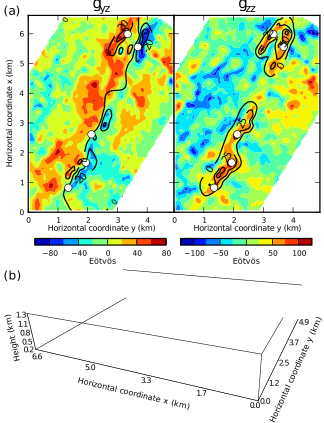
\includegraphics[width=\columnwidth]{real/quadrilatero/fig/quadrilatero}
     %\vspace{-0.6cm}
    \caption{Application to gravity gradient tensor data from the
        Quadril\'atero Ferr\'ifero, Brazil. (a) Observed (colored contours) and
        predicted (black contour lines) $g_{yz}$ and $g_{zz}$ components of
        the gravity gradient tensor. White dots show the horizontal locations
        of the five seeds used in the inversion. (b) Perspective view of the
        estimated density-contrast distribution.
        Red prisms have density contrast of $1.0\ \mathrm{g/cm}^3$.
        Prisms with density contrast of $0\ \mathrm{g/cm}^3$ are not shown.
    \label{fig:qf}}
    %\vspace{-0.5cm}
\end{figure}


\section{Acknowledgments}

\begin{sloppypar}
We thank Vale for permission to use the data of the Quadril\'atero Ferr\'ifero.
We acknowledge the use of software matplotlib by \citet{Hunter2007} and Mayavi
by \citet{Ramachandran2011} for 2D and 3D graphics, respectively.
The authors were supported in this research by a fellowship (VCFB) from
Conselho Nacional de Desenvolvimento Cient\'ifico e Tecnol\'ogico (CNPq) and a
scholarship (LU) from Coordena\c{c}\~ao de Aperfei\c{c}oamento de Pessoal de
N\'ivel Superior (CAPES), Brazil.
Additional support for the authors was provided by the Brazilian agencies CNPq
(grant 471693/2011-1) and FAPERJ (grant E-26/103.175/2011).
\end{sloppypar}

\begin{figure}[htb]
    %\vspace{-6.5cm}
    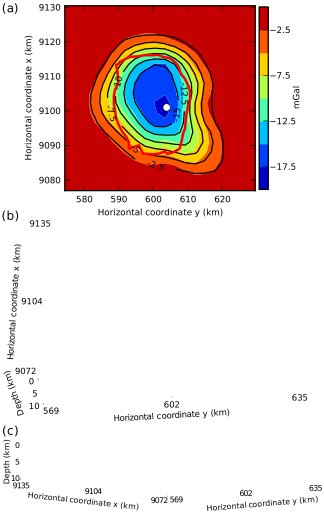
\includegraphics[width=\columnwidth]{real/redencao/fig/redencao}
     %\vspace{-0.6cm}
    \caption{Application to the Bourguer anomaly data of the Reden\c{c}\~ao
        granite, Brazil.
        (a) Observed (colored contours) and predicted (black contour
        lines) data. The white dot shows the horizontal location of the single
        seed used in the inversion. (b-c) Perspective views of the estimated
        density-contrast distribution.
        Blue prisms have density contrast of $-0.09\ \mathrm{g/cm}^3$.
        Prisms with density contrast of $0\ \mathrm{g/cm}^3$ are not shown.
        The red line in a-c represents the true outcropping portion of the
        pluton. 
    \label{fig:redencao}}
    %\vspace{-0.5cm}
\end{figure}

\newpage
% style file is seg.bst
\bibliographystyle{seg}  
\onecolumn
\nobibliography{seg2012}
%\bibliography{seg2012}

\end{document}
